%% P--StwoS.tex
%% Sample file to use for P--S articles prepared in LaTeX
%% For two column P--S articles
%% Version1: Apr 15, 2008
%% Version2: Oct 04, 2013

%% BASIC CLASS FILE
\documentclass{pnastwo}

%% ADDITIO--L OPTIO--L STYLE FILES Font specification

%\usepackage{pnastwoF}
\usepackage{color,capt-of,lipsum}
%\usepackage[square,sort,comma,numbers]{natbib}


%% OPTIO--L MACRO DEFINITIONS
\def\s{\sigma}
\newcommand{\eref}[1]{(\ref{#1})}
\newcommand{\tableref}[1]{Table \ref{#1}}
\newcommand{\figref}[1]{Fig.~\ref{#1}}
\newcommand{\appref}[1]{Appendix \ref{#1}}
\newcommand{\sectionref}[1]{Section \ref{#1}}

\definecolor{Red}{RGB}{255,0,0}
\newcommand{\red}[1]{\textcolor{Red}{#1}}

%%%%%%%%%%%%
%% For P--S Only:
\url{www.pnas.org/cgi/doi/10.1073/pnas.0709640104}
\copyrightyear{2015}
\issuedate{Issue Date}
\volume{Volume}
\issuenumber{Issue Number}
%\setcounter{page}{2687} %Set page number here if desired
%%%%%%%%%%%%

\begin{document}

\title{Subjectivity predicts adjective ordering preferences}

\author{Gregory Scontras\affil{1}{Department of Psychology, Stanford University, Stanford, CA 94305},
Judith Degen\affil{1}{},
\and
Noah D.\ Goodman\affil{1}{}}

\contributor{Submitted to Proceedings of the National Academy of Sciences
of the United States of America}

%%%Newly updated.
%%% If significance statement need, then can use the below command otherwise just delete it.
\significancetext{Speakers and listeners exhibit robust ordering preferences when it comes to modification involving more than one adjective. We present experimental and corpus results showing that these preferences track the subjectivity of the adjectives at play, such that less subjective adjectives occur closer to the nouns they modify. Rather than representing these preferences as a fully specified ranking according to lexical items or semantic classes, we show that ordering preferences more likely emerge from a desire to place more informative, less subjective content closer to the substanstive head of a nominal construction (i.e., closer to the modified noun).}

\maketitle

\begin{article}
\begin{abstract}
{Abstract here\ldots}
\end{abstract}

\keywords{language | ordering preferences | subjectivity | faultless disagreement}

%\abbreviations{SAM, self-assembled monolayer; OTS, octadecyltrichlorosilane}

\dropcap{L}inguistic competence encompasses a broad swath of information that determines the language we speak. The information, grammar, is ``mentalistic'' \cite{chomsky1965}; we observe it through the regularities in behavior of speakers and speech communities. Here we take up one such regularity, adjective ordering. Speakers and listeners exhibit strong preferences when two or more adjectives are used to modify a noun, as in ``the big blue box'' or ``the good smooth purple plastic chair.'' Deviate from the preferred order, and the construction becomes marked: something feels particularly unwieldy about ``the blue big box,'' even more so with ``the plastic good purple smooth chair.'' Indeed, for any string of pre-nominal adjectives, chances are their order is non-arbitrary. The question is why.

Even more intriguing than their robustness in English is the cross-linguistic regularity of these preferences; not only do we find adjective ordering preferences across the world's languages, we continually find the \emph{same} preferences. Hungarian (Uralic), Telugu (Dravidian), Mandarin Chinese, and Dutch are just a handful of the languages reported to have the same ordering preferences as English \cite{dixon1982,sproatshih1991,martin1969competence,hetzron1978,lapollahuang2004}. These preferences determine the linear distance of an adjective from the noun it modifies, both pre- and post-nominally. In languages like Selepet (Papuan) and Mokilese (Micronesian) with post-nominal adjectives (i.e., where adjectives follow nouns), these preferences are preserved in the reverse \cite{dixon1982,sproatshih1991}. 

There have been two styles of approaches to the investigation of adjective ordering preferences. The first is what we call the ``psychological'' approach, which advances the idea that aspects of  adjectives' meaning determine their relative order. But which aspects of meaning? Kicking off the enterprise in 1898, Sweet proposed that adjectives which are more closely connected with the noun in meaning occur closer to the noun, and that adjectives with a more specialized meaning occur closer to the noun \cite{sweet1898}. Similarly, Whorf proposed that adjectives describing more ``inherent'' properties occur closer to the noun \cite{whorf1947}. Ziff proposed that adjectives with less context-dependent meaning occur closer to the noun, and that adjectives that felicitously describe a narrower set of nouns occur closer to the noun \cite{ziff1960}. The proposals circle around similar aspects of adjective meaning in their account of ordering preferences; unfortunately, operationalizing metrics like meaning distance, specificity, inherence, and context-dependence is not a trivial task (but see the attempts in \cite{martin1969determinants}). More importantly, for a psychological theory of ordering preferences to get off the ground, we would need a mapping hypothesis between the relevant aspects of meaning and the cognitive processes that attend to them.

As part of a larger project mapping the syntax and semantics of adjectives (a ``cartographic'' approach, one could say), in the 1980s the literature on ordering preferences marks a turn away from the psychological determinants of ordering preferences, and toward a universal syntactic hierarchy of semantic classes of adjectives. In contrast to the psychological approaches, these ``grammatical'' approaches are primarily concerned with uncovering language-internal structure by which to organize ordering preferences. Grammatical approaches assume that ordering preferences are universal and hard-coded in the grammar; our job is simply to uncover them. 
Building on the orderings and semantics classes proposed by Dixon \cite{dixon1982}, Cinque advanced a fully syntactic account of ordering preferences under which different semantic classes of adjectives populate dedicated syntactic categories which inhabit specialized projections in the syntactic tree \cite{cinque1994}. For example, color adjectives project a Color Phrase, shape adjectives project a Shape Phrase. The Shape Phrase syntactically dominates the Color Phrase; left-branching structure has hierarchical dominance result in linear precedence. The ultimate source of this rigid structure is left up for grabs; what matters is a comprehensive and deterministic theory of the facts.


Where psychological approaches are focused on the mind from which these preferences emerge, grammatical approaches target the language in which they operate---a system which the linguistics tradition has described in terms of structural rules---appealing to properties of language to map, as it were, the terrain of adjective structure. Our approach synthesizes strategies from the psychological approach, probing the principles that underlie these preferences, and from the grammatical approach, using semantic classes of adjectives to structure and inform our investigation. Rather than falling back on a rigid syntax, we advance the hypothesis that adjective subjectivity stands as the main determinant of these preferences. Less subjective adjectives are reliably more informative; there is little question about what the speaker meant to communicate. These more informative adjectives occur closer to the substantive head on the nominal projection, that is, to the modified noun.

To test the hypothesis that adjective subjectivity predicts ordering preferences, we validated two key empirical constructs: 1) the ordering preferences themselves, and 2) an adjective's subjectivity. With reliable estimates of both, we then evaluated the predictive power of subjectivity in adjective ordering preferences.

\section{Ordering preferences}

We began by measuring the ordering preferences for which we must account. We selected a sample of 26 relatively frequent adjectives from seven different semantic classes discussed in the grammatical literature (size, quality, age, texture, shape, color, material) and elicited naturalness judgments on adjective-adjective-noun object descriptions, permuting the relative order of the adjectives. Participants indicated which ordering of an object description (e.g., ``the big red apple'' vs.\ ``the red big apple'') sounded more ``natural'' (see \emph{Materials and Methods} for details).

On the basis of these naturalness ratings, we computed for each adjective-adjective pairing its preferred, canonical order (i.e., the order that sounded more natural to participants). We then determined how often an adjective from a given semantic class occurred first in a preferred  configuration; Fig.\ \ref{results} (\emph{preference}) plots these mean preference scores, where a value of 1 signals that a class's adjectives always occur first in preferred adjective-adjective-noun orderings, and a value of 0 indicates that a class's adjectives always occur second, closest to the noun. This preferred distance measure closely tracks ordering hierarchies reported in the literature \cite{dixon1982,sproatshih1991}.

To independently validate our behavioral measure of ordering preferences, we conducted a corpus study on the same 26 adjectives and measured their mean distance from the noun in phrases with either two or three adjectives. We extracted all such cases from the Switchboard Corpus and the British National Corpus (see \emph{Materials and Methods} for details). Mean distance from the noun for each adjective class is shown in Fig.~\ref{results} (\emph{corpus}); higher values indicate that adjectives from the specified class tend to appear farther from the modified noun. The corpus measure replicates the qualitative pattern we measured in our naturalness experiment; quantitatively, the two measures are highly correlated ($r^{2}=0.72$, 95\% CI [0.39, 0.86]; Fig.~\ref{corpus-naturalness}). Our naturalness ratings thus serve as valid empirical constructs of speakers' ordering preferences.

\section{Subjectivity}

The extent to which two people can disagree about a description without one necessarily being wrong determines the subjectivity of that description. To  establish an ecologically valid measure of adjective subjectivity, we operationalized it as the potential for faultless disagreement between two speakers. We had participants evaluate whether two speakers could both be right while asserting conflicting object descriptions. For example, an experimental trial would have Mary assert, ``That apple is old,'' then have Bob counter with ``That apple is not old;'' 
participants rated whether both Mary and Bob could be right, or whether one of them must be wrong (see \emph{Materials and Methods} for more details). This measure, the faultless disagreement potential for the adjective at issue, serves as our empirical construct of adjective subjectivity. Fig.\ \ref{results} (\emph{faultless}) plots these scores by adjective class, where a value of 1 signals that a class's adjectives are always amenable to faultless disagreement, and a value of 0 indicates that a class's adjectives are never amenable to faultless disagreement.

We validated our faultless disagreement measure in a separate paradigm with a more direct yet potentially less ecologically valid measure of adjective subjectivity: participants were asked explicitly to rate the ``subjectivity'' of object descriptions like ``old apple.'' The results of this method (Fig.~\ref{results}, \emph{subjectivity}) were highly correlated with our faultless disagreement scores ($r^{2} = 0.89$, 95\% CI [0.81, 0.93]; Fig.~\ref{subjectivity-faultless}), suggesting that the measures they invoke converge in their estimation of adjective subjectivity. We therefore take our faultless disagreement scores as valid empirical constructs of subjectivity.

\section{Predicting adjective order}

To evaluate the power of subjectivity in predicting adjective ordering preferences, we compared our naturalness ratings to the faultless disagreement scores. We  computed a subjectivity difference score for each class configuration (i.e., an ordered pairing of two adjective classes, \textsc{class1}-\textsc{class2}) by subtracting the mean faultless disagreement score for \textsc{class2} from the mean faultless disagreement score for \textsc{class1}. Higher difference scores indicate that the adjective class closer to the noun is less subjective than the class farther away. Fig.~\ref{naturalness-faultless} plots naturalness ratings  against these faultless disagreement difference scores; the two measures are highly correlated ($r^2$ = 0.82, 95\% CI [0.72, 0.89]), strongly supporting the hypothesis that less subjective adjectives occur more closely to the noun.

\section{Discussion}

Adjective ordering preferences have received considerable attention throughout the history of generative grammar and cognitive psychology, owing to their remarkable stability within and across languages. Something so robust, the reasoning goes, must evidence a deep principle of the cognitive architecture that shapes language. Yet while descriptions of the phenomenon abound, an explanation continues to prove elusive. Grammatical theories that posit a rigid syntax of adjective classes offer little more than a reminder of the facts, and psychological approaches stumble when it comes to operationalizing the specific aspects of adjective meaning at play. 

In our investigation, we established two empirical constructs: the preferences themselves, which we measured using naturalness ratings and validated with corpus counts; and adjective subjectivity, which we operationalized as potential for faultless disagreement and validated with a direct measure. Our findings suggest a clear path forward: an adjective's semantics can indeed predict its distance from the modified noun, such that less subjective adjectives occur linearly closer to nouns they modify. Rather than representing these preferences as a rigid, fully specified ranking according to semantic classes or syntactic projections, these results demonstrate that ordering preferences more likely emerge from a desire to place less subjective, more informative content closer to the substantive head of a nominal construction (i.e., closer to the modified noun).



\newpage

\begin{materials}
\section{Corpus counts} 

We used TGrep2 \cite{rohde2005} and the TGrep2 Database Tools \cite{degenjaeger-tdt} to extract all ``A A N" and ``A A A N" NPs that contained one of the 26 adjectives in Table \ref{TABLREFER} from the Penn Treebank subset of the Switchboard corpus of telephone dialogs \cite{godfrey1992} as well as from the spoken and the written portions of the British National Corpus (\red{REF}). There were a total of 35,721 cases. For these cases, we computed the distance of each occurrence of our 26 target adjectives from the noun, yielding results for a total of 39,199 adjectives (180 from Switchboard, 2,232 from the spoken BNC, 36,787 from the written BNC).  See \tableref{tab:adjdist} for the distribution of cases over adjective classes.

\begin{table}
	\caption{Distribution of cases extracted from corpora over adjective classes}
	\begin{tabular}{l c c c c c c c}
	\textbf{Class} & age & size & color & quality & texture & material & shape \\
	\textbf{Count} & 15,688 & 11,576 & 5,024 & 3,790 & 1,720 & 1, 183 & 218 \\
	\textbf{Proportion} & .40 & .30 & .13 & .10 & .04 & .03 & .01
	\end{tabular}
\label{tab:adjdist}
\end{table}


For each adjective class, mean distance from the noun was computed (where position directly preceding the noun was coded as 0, the position preceding that as 1, etc.). The resulting by-class mean distances are shown in \figref{fig:distance}. To determine which differences between adjective classes are meaningful differences, we conducted Bonferroni-corrected pairwise t-tests. All differences were significant at the .0001 level except for the difference between color and shape (significant at the .04 level) and the difference between size and quality (not significant). See \tableref{tab:bonferronicorpus} for a summary. These results suggest that except for the exact position of size and quality, the order established in \figref{fig:distance} is real.

\begin{table}
\caption{Pairwise comparisons between adjective classes using t-tests with Bonferroni correction}

\begin{tabular}{l l l l l l l}
       &  age & color & material & quality & shape & size\\
color &     $<$.0001 &    --   &    --   &   -- &   --  & --\\
material &  $<$.0001 &  $<$.0001 &      --  &    -- &   -- &  --\\
quality &   $<$.0001 & $<$.0001 &         $<$.0001 &      --  &  -- &  --\\
shape &     $<$.0001 & $<$.04 &        $<$.0001 &  $<$.0001 &    -- &  --\\
size &      $<$.0001 & $<$.0001 &        $<$.0001 &  $<$.76 &    $<$.0001 &   --\\
texture &   $<$.0001 & $<$.0001 &       $<$.0001 &  $<$.0001 &    $<$.0001 &    $<$.0001
\end{tabular}
\label{tab:bonferronicorpus}
\end{table}

Pairwise comparisons using t tests with bonferroni correction
         age     color   material quality shape   size   
         color    < 2e-16 -       -        -       -       -      
         material < 2e-16 8.9e-05 -        -       -       -      
         quality  < 2e-16 < 2e-16 < 2e-16  -       -       -      
         shape    < 2e-16 0.032   1.3e-05  < 2e-16 -       -      
         size     < 2e-16 < 2e-16 < 2e-16  0.636   < 2e-16 -      
         texture  2.1e-13 < 2e-16 < 2e-16  < 2e-16 1.9e-10 < 2e-16

\section{Experiment 1a: Faultless Disagreement}
Something about our methods and how we ran the experiment


Pairwise comparisons using t tests with bonferroni correction
		         age     color   material quality shape   size   
         color    < 2e-16 -       -        -       -       -      
         material < 2e-16 0.00161 -        -       -       -      
         quality  7.6e-06 < 2e-16 < 2e-16  -       -       -      
         shape    < 2e-16 0.25546 1.00000  < 2e-16 -       -      
         size     2.8e-10 < 2e-16 < 2e-16  1.00000 < 2e-16 -      
         texture  1.00000 < 2e-16 < 2e-16  0.00011 < 2e-16 1.1e-07

\begin{table}
	\caption{Adjectives and nouns used in experimental stimuli.}
	\begin{tabular}{@{\vrule height 10.5pt depth2pt  width0pt}llllll}
	\textbf{adjective}	&	\textbf{class}	&	\textbf{adjective}	&	\textbf{class}	&	\textbf{noun}	&	\textbf{class}	\\ \hline
old	&	age	&	good	&	quality	&	apple	&	food	\\
new	&	age	&	bad	&	quality	&	banana	&	food	\\
rotten	&	age	&	round	&	shape	&	carrot	&	food	\\
fresh	&	age	&	square	&	shape	&	cheese	&	food	\\
red	&	color	&	big	&	size	&	tomato	&	food	\\
yellow	&	color	&	small	&	size	&	chair	&	furniture	\\
green	&	color	&	huge	&	size	&	couch	&	furniture	\\
blue	&	color	&	tiny	&	size	&	fan	&	furniture	\\
purple	&	color	&	short	&	size	&	TV	&	furniture	\\
brown	&	color	&	long	&	size	&	desk	&	furniture	\\
wooden	&	material	&	smooth	&	texture	\\				
plastic	&	material	&	hard	&	texture	\\				
metal	&	material	&	soft	&	texture	\\													
	\end{tabular} \label{stim-table}\caption{Adjectives and nouns used in experimental stimuli.}
\end{table}

\section{Experiment 1b: Subjectivity}

\section{Experiment 2: Ordering preferences}
We recruited 50 participants through Amazon.com's Mechanical Turk crowd-sourcing service. Participants were compensated for their participation.

Participants were asked to indicate which of two descriptions of an object sounded more natural. Each description featured a noun modified by two adjectives, for example ``the red small chair'' or ``the small red chair''. Description pairs contained the same words, with relative adjective order reversed. Descriptions were random combinations of two adjectives and a noun from the list in Table \ref{stim-table} (compiled via the procedure described in Section \ref{corpus}), with the constraint that no description contained adjectives from the same adjective class.
On each trial, participants indicated which description sounded more natural by adjusting a slider whose endpoints were labeled with the competing descriptions; an example trial appears in Fig.\ \ref{order-trial}.

\begin{figure}[h!]
	\centering
	\fbox{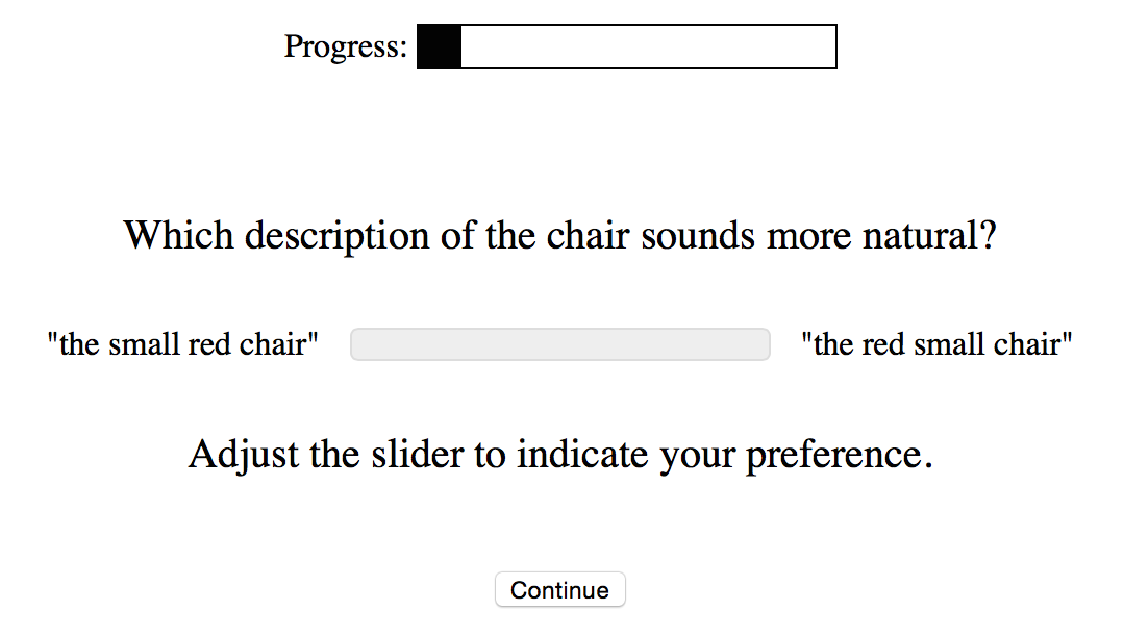
\includegraphics[width=.8\linewidth]{images/order_trial.eps}}
	\caption{Example trial from Expt.\ 1; participants indicated the more natural of two adjective-adjective-noun descriptions on a sliding scale.}\label{order-trial}
\end{figure}

Only native speakers of English with IP addresses located within the United States were included in the analyses; we analyzed data from 45 participants.



\begin{table}
	
\begin{tabular}{lllllll}
	   &    age & color & material & quality & shape & size  \\ 
color &		\textbf{$<$0.001} & -       & -        & - & - & - \\      
material &	\textbf{$<$0.001} & 1.00 & -        & - & - & - \\      
quality & 	0.98 & \textbf{$<$0.001} & \textbf{$<$0.001}  & - & - & - \\      
shape & 	1.00 & \textbf{$<$0.05} & \textbf{$<$0.001}  & \textbf{$<$0.05} & - & - \\     
size & 		\textbf{$<$0.001} & \textbf{$<$0.001} & \textbf{$<$0.001}  & 0.11 & \textbf{$<$0.001} & - \\     
texture & 	1.00 & \textbf{$<$0.001} & \textbf{$<$0.001}  & 1.00 & 0.30 & \textbf{$<$0.001}
\end{tabular}
\caption{Pairwise comparisons using t tests with Bonferroni correction \red{---would be nicer to have adjectives in the order of the plot for ease of readability; also, currently wrong numbers}}
\end{table}

\textbf{$<$0.001}



\end{materials}

\begin{acknowledgments}
This work was supported in part by Office of Naval Research Grant N000141310788 (to N.D.G.).
\end{acknowledgments}

\begin{thebibliography}{10}
	\bibitem{chomsky1965}
	N.~Chomsky, {\em Aspects of the Theory of Syntax} (1965).

	\bibitem{sweet1898}
	H.~Sweet, {\em A New English Grammar} (1898).
	
	\bibitem{bloomfield1933}
	L.~Bloomfield, {\em Language} (1933).
	
	\bibitem{sproatshih1991}
	R.~Sproat and C.~Shih, 1991. {\em The cross-linguistic distribution of adjective ordering restrictions}, Interdisciplinary approaches to language: Essays in honor of S.-Y.~Kuroda (1991), pp.~565--593.
	
	\bibitem{martin1969competence}
	J.~E.~Martin, {\em Some Competence-Process Relationships in Noun Phrases with Prenominal and Postnominal Adjectives}, Journal of Verbal Learning and Verbal Behavior, 8 (1969), pp.~471--480. 	
	
	\bibitem{wulff2003}
	S.~Wulff, {\em A multifactorial corpus analysis of adjective order in English},
	International Journal of Corpus Linguistics, 8 (2003), pp.~245‒-282.
	
	\bibitem{ziff1960}
	P.~Ziff, {\em Semantic Analysis} (1960).
	
	\bibitem{martin1969determinants}
	J.~E.~Martin, {\em Semantic Determinants of Preferred Adjective Order}, Journal of Verbal Learning and Verbal Behavior, 8 (1969), pp.~697--704. 
	
	\bibitem{martin1970}
	J.~E.~Martin, {\em Adjective Order and Juncture}, Journal of Verbal Learning and Verbal Behavior, 9 (1970), pp.~379--383. 
	
	\bibitem{haiman1985}
	J.~Haiman, {\em Natural Syntax} (1985).
	
	\bibitem{dixon1982}	
	R.~M.W.~Dixon, {\em Where have all the adjectives gone?, and other essays in semantics and syntax} (1982).
	
	\bibitem{cinque1994}
	G.~Cinque, {\em On the evidence for patial N-movement in the Romance DP}, Paths towards Universal Grammar. Studies in honor of Richard S.~Kayne (1994), pp.~85--110.
	
	\bibitem{scott2002}
	G.-J.~Scott, {\em Stacked adjectival modification and the structure of nominal phrases}, The Cartography of Syntactic Structures (2002), pp.~91--120.
	
	\bibitem{rohde2005}
	D.~Rohde, TGrep2 User Manual (2005).
	
	\bibitem{degenjaeger-tdt}
	J.~Degen and T.F.~Jaeger, The TGrep2 Database Tools (2011).
	
	\bibitem{godfrey1992}
	J.~Godfrey and E.~Holliman and J.~McDaniel, {\em Switchboard: A Telephone Speech Corpus for Research and Development}, Proceedings of ICASSP-92 (1994),
	pp.~517--520.
	
	\bibitem{diciccioefron1996}
	T.~DiCiccio and B.~Efron, {\em Boostrap confidence intervals (with discussion)}, Statistical Science, 11 (1996), pp.~189--228.
\end{thebibliography}


\end{article}

\begin{figure*}
	\centering
	{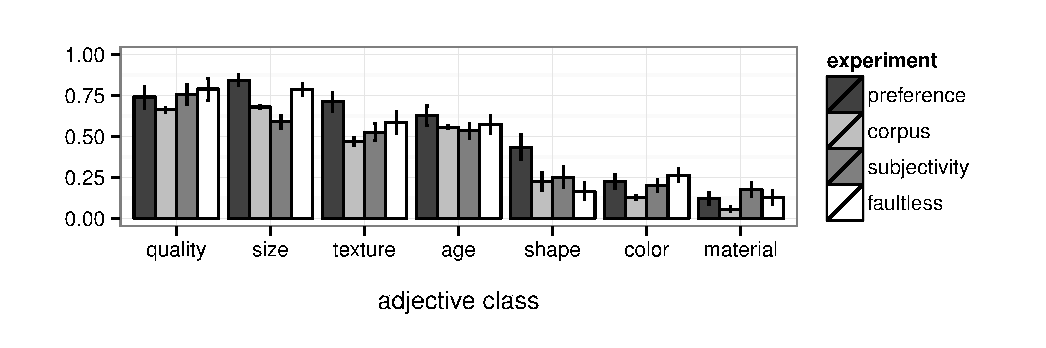
\includegraphics[width=.75\linewidth]{plots/expt_results.eps}}\par
	%\vspace{-10pt}
	\caption{Mean distance from noun inferred from naturalness ratings (preference), mean distance from noun calculated from corpus counts (corpus),  mean faultless disagreement ratings (subjectivity), and mean subjectivity ratings (subjectivity) for adjectives grouped by their semantic class. Error bars represent bootstrapped 95\% confidence intervals \cite{diciccioefron1996}.}\label{results}
\end{figure*}

\begin{figure}
	\centering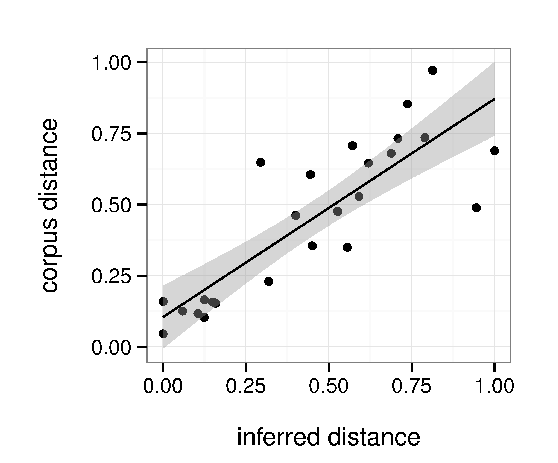
\includegraphics[width=2.15in]{plots/corpus-naturalness.eps}
	\caption{Mean distance from noun calculated from corpus counts plotted against mean distance from noun inferred from naturalness ratings for each of the 26 adjectives tested.}\label{corpus-naturalness}
\end{figure}

\begin{figure}
	\centering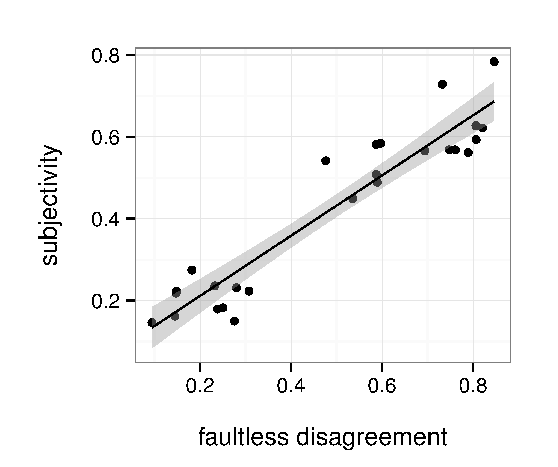
\includegraphics[width=2.15in]{plots/subjectivity-faultless.eps}
	\caption{Mean subjectivity ratings plotted against mean faultless disagreement ratings for each of the 26 adjectives tested.}\label{subjectivity-faultless}
\end{figure}

\begin{figure}
	\centering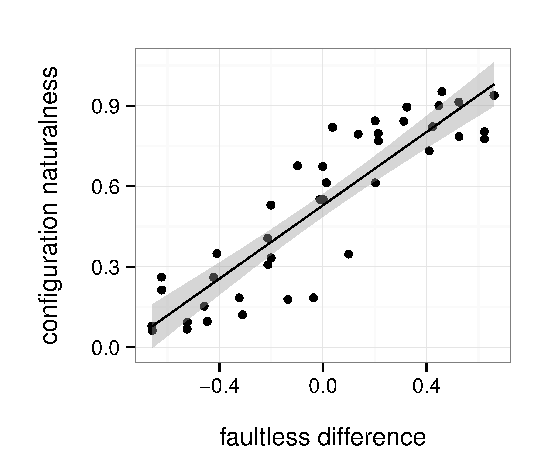
\includegraphics[width=2.15in]{plots/naturalness-faultless.eps}
	\caption{Mean naturalness ratings plotted against subjectivity difference scores for each pair of adjective classes.}\label{naturalness-faultless}
\end{figure}


\end{document}






We then compared these naturalness judgments with the subjectivity scores.

For each pair of adjective classes, we determine the preferred ordering on the basis of the ratio of ratings for the each order. Ratio scores greater than 1 indicate the preferred ordering; these ratio scores for the preferred orderings are plotted in Fig.\ \ref{order-ratio}.

\begin{figure}[h]
	\centering
	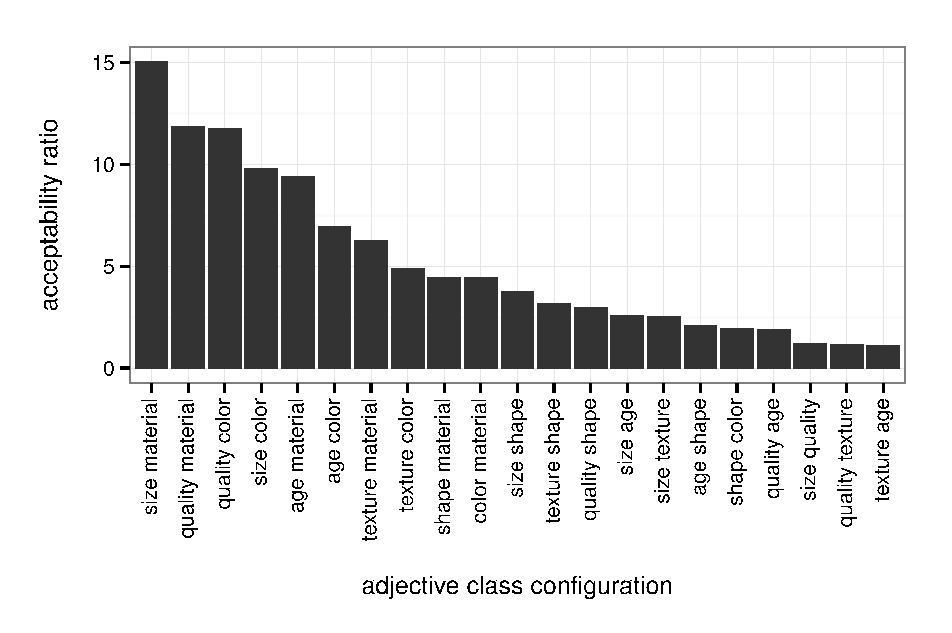
\includegraphics[width=.95\linewidth]{plots/order_ratio.eps}
	\caption{Accpetability ratios for the preferred adjective class orderings.}\label{order-ratio}
\end{figure}

On the basis of these preferred orderings, we may calculate the average distance from noun for each class, plotted in Fig.\ \ref{class-distance}. Comparing Fig.\ \ref{class-distance} with the corpus-based distance scores reported in Fig.\ \ref{distance-from-noun} confirms the reliability of the current paradigm: we replicate near exactly the qualitative order of adjective class distance from noun. 

\begin{figure}[h]
	\centering
	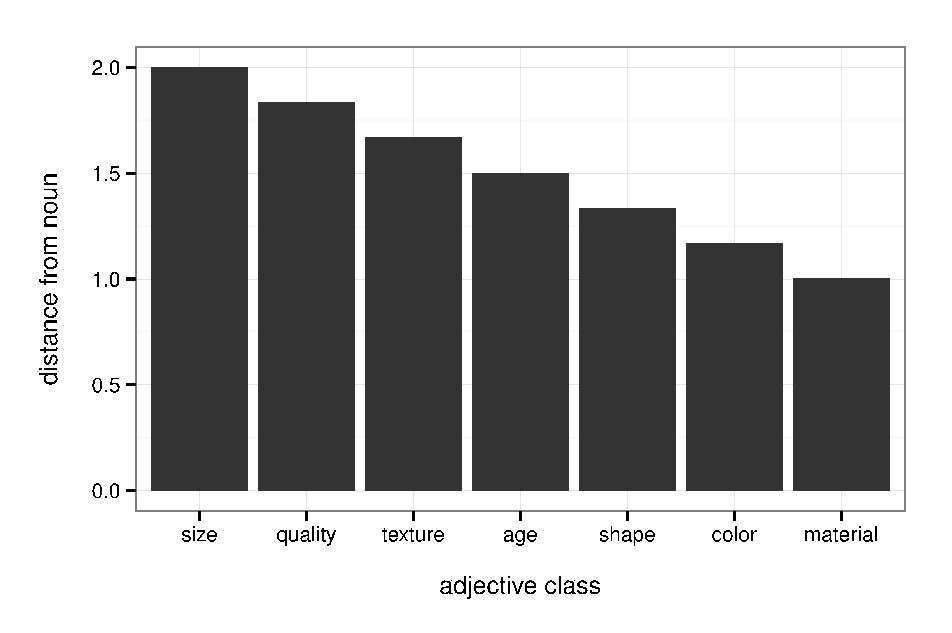
\includegraphics[width=.95\linewidth]{plots/class_distance.eps}
	\caption{Average distance from noun for each adjective class calculated from order preference ratings.}\label{class-distance}
\end{figure}

We may infer the order preferences in \ref{expt-inferred-order-preferences} (cf.\ the preferences inferred from corpus counts in \ref{inferred-order-preferences} above).
\be
size > quality > age > texture > shape > color > material\label{expt-inferred-order-preferences}\ee 


To infer an ordering that could be compared with orders reported in the literature, we conducted pairwise Bonferroni-corrected comparisons on the mean distance-from-noun scores calculated in Fig.~\ref{results}; these comparisons yielded the following ordering preferences:
\be size \geq quality > age > texture > shape > color > material \label{inferred-order-preferences}\ee
Our inferred order closely tracks previous reports (cf.~the orders in \ref{dixon-order},\ref{ss-order}). Taking corpus counts as a proxy for preferences in production such that preferred orders get produced more often, we thus find support for active and stable ordering preferences in speakers. However, the source of these preferences and the level of representation that they target remains a mystery: the stable ordering observed in corpora could emerge from superficial production pressures (e.g., relative frequency or accessibility), rather than deep cognitive principles. To test the awareness and thus robustness of these preferences in language, we next shifted focus from speakers to listeners.



replicated the qualitative order inferred from the corpus counts in the first experiment. We therefore conclude that, like speakers, listeners possess active and stable ordering preferences, suggesting that the source of these preferences concerns more than just pressures during production. And given the remarkable similarity, both qualitative and quantitative, between the results of the current experiment and the distance measures computed in Experiment 1, we furthermore conclude that generalizing to the level of semantic classes proves useful in characterizing the phenomenon of interest.

1) whether they exhibit ordering preferences, and 2) what those preferences are. We then entertained the hypothesis that aspects of adjective meaning shape ordering preferences. Our intuition, which we validate empirically, was that adjective subjectivity---how easy it is for different speakers to arrive at different judgments for the same property---predicts ordering preferences. 






Fig.~\ref{results} (subjectivity) plots mean faultless disagreement ratings for adjectives and their respective classes. These subjectivity scores closely track the distance measures from Experiments 1 and 2, with the exception that color adjectives are judged more subjective than shape adjectives, yet color adjectives tend to appear closer to the modified noun (e.g., ``the round purple desk'' vs.~``the purple round desk''). Curiously, the relative subjectivity of shape vs.~color adjectives was one of the areas where our two measures pulled apart; with the direct ``subjectivity'' measure, shape is rated higher than color, in line with the distance measures from Experiments 1 and 2.



, owing to its remarkable stability within and across languages. Something so robust, the reasoning goes, must evidence a deep principle of the cognitive architecture that shapes language. Yet while descriptions of the phenomenon abound, an explanation continues to prove elusive. 

\section{Background}
Linguists have been aware of adjective ordering preferences (or restrictions; often abbreviated ``AOR'') for well over a century now \cite{sweet1898,bloomfield1933}. Even more curious than their robustly attested status in English is their cross-linguistic regularity, observed in languages as far-flung as Celtic \cite{sproatshih1991} and Indonesian \cite{martin1969competence}. 

We review each style of approach in turn, then discuss how the approach we take here adopts aspects of both.
\subsection{Psychology}
The descriptions of ordering preferences that have so far been proffered are nearly as diverse as the principles to which they appeal (see \cite{wulff2003} for a comprehensive review of the many potential factors contributing to adjective order in production). 


Haiman \cite{haiman1985} proposes instead that adjective ordering preferences are symptomatic of a more general semiotic coding strategy called ``diagrammatic iconicity'' (i.e., non-arbitrary form-meaning mappings). This theory holds that distance relations in semantic space may be mapped onto distance relations in syntactic space, such that adjectives further from the noun in meaning occur farther from the noun syntactically. To move from a philosophical to a psychological theory, however, Haiman's proposal would require specifying just how more definite, less context-sensitive adjectives are closer in meaning to the nouns they modify. Indeed, a semiotic approach like Haiman's harkens back to Sweet's original description of the phenomenon of ordering preferences, namely that adjectives closer in meaning to the noun occur linearly closer to it \cite{sweet1898}. The question remains: in what sense are nominal and adjectival meaning comparable, and why should distance in meaning relate to linear distance in production?

To summarize, psychological approaches to adjective ordering focus on the aspects of meaning and cognition that would generate the observed preferences. They contrast with grammatical approaches, which focus instead on the adjectives themselves. We turn to them next.

\subsection{Grammar}
These classes divide on the basis of the properties named by the adjectives that populate them (e.g., size, shape, color). At the heart of this enterprise is R.~Dixon \cite{dixon1982}, who argues that by prioritizing the study of adjective semantics, we may gain insight into properties of their syntactic distribution; one such property that semantics is meant to inform concerns their relative order in multi-adjective strings. After surveying a wealth of languages, Dixon arrives the adjective classes (or ``types'') in \ref{dixon-order}.\footnote{Here are some representative examples of Dixon's semantic classes:\\ \textit{dimension}: ``big'', ``small''; \textit{physical property}: ``hard'', ``heavy''; \textit{speed}: ``fast'', ``slow''; \textit{human propensity}: ``happy'', ``clever''; \textit{age}: ``new'', ``young''.} He furthermore ranked these classes according to their distance from the noun they modify; in multi-adjective strings, higher ranked adjectives occur farther from the modified noun.
\[
dimension > physical\ property > speed > 
\]
\be human\ propensity > age > color\label{dixon-order}\ee
While the ranking in \ref{dixon-order} is meant to characterize English preferences, Dixon notes that evidence of this ranking also surfaces in Hungarian (Uralic) and Telugu (Dravidian). Interestingly, in Selepet (Papuan), where adjectives typically occur post-nominally, the order in \ref{dixon-order} is preserved in the reverse, such that higher ranked adjectives occur farther to the right of the modified noun. 

Using a smaller and perhaps more transparently labeled set of semantic classes, \cite{sproatshih1991} proposed the ranking in \ref{ss-order}.
\be quality > size > shape > color > provenance\label{ss-order}\ee
In addition to English, the authors show that this ordering surfaces with pre-nominal adjectives in Mandarin Chinese, Dutch, and Kannada (Dravidian). And in Mokilese (Micronesian), a language like Selepet with post-nominal multi-adjective strings, the ordering in \ref{ss-order} is once again preserved in the reverse. Languages from all over the world exhibit ordering preferences, and, whether or not adjectives occur pre- or post-nominally, these preferences attend to distance from the modified noun.\footnote{For evidence of these preferences in yet more languages, see \cite{martin1969competence,hetzron1978,lapollahuang2004}.)}

In addition to the well-behaved languages mentioned above, Sproat and Shih discuss the potentially puzzling case of Celtic languages. In Irish and Welsh, adjectives occur post-nominally and there are preferred adjective orders (cf. Mokilese and Selepet), but the preferences preserve the English-like ranking and thereby reverse the scale in \ref{ss-order}: higher-ranked adjectives occur  \emph{closer} to the noun. The authors explain this pattern by appealing to a core property of Celtic VSO languages: both verbs and noun are ``fronted,'' moving to a phrase-initial position \cite{sproat1985,guilfoyle1987}. Assuming that Celtic nouns begin to the right of the adjectives that modify them, then front to a phrase-initial position to their left, the ordering preferences in Celtic languages evidence a planning trajectory that orders adjectives before finalizing the placement of the noun they modify; distance from the modified noun---albeit at an intermediate stage of planning---is still the key to the process.

\footnote{The class ranking Cinque uses as the basis for his syntactic proposal follows the ranking from \cite{sproatshih1991} in \ref{ss-order}: 
	\be quality > size > shape > color > nationality\label{cinque-order}\ee}
For example, 



\subsection{The upshot} Our approach to the investigation of ordering preferences synthesizes strategies from the psychological approach, probing the principles that underlie these preferences, and from the grammatical approach, using descriptive adjective classes to structure and inform our exploration and hypothesis. We selected a class of relatively frequent adjectives from a range of semantic classes and asked 1) whether they exhibit ordering preferences, and 2) what those preferences are. We then entertained the hypothesis that aspects of adjective meaning shape ordering preferences. Our intuition, which we validate empirically, was that adjective subjectivity---how easy it is for different speakers to arrive at different judgments for the same property---predicts ordering preferences. Less subjective adjectives are reliably more informative; there is little question about what the speaker meant to communicate. These more informative adjectives occur closer to the substantive head on the nominal projection, that is, to the noun.

\section{Experiment 1: Corpus counts}



\section{Experiment 2: Ordering preferences}
Finding evidence for ordering preferences in speakers, we then asked whether meta-linguistic awareness of these preferences exists in listeners. Finding as much, we would have evidence for the psychological reality of ordering preferences. To that end, we elicited naturalness judgments on adjective-adjective-noun object descriptions, permuting the relative order of the adjectives. Participants indicated which ordering of an adjective-adjective-noun object description (e.g., ``the big red apple'' vs.\ ``the red big apple'') sounded more natural. We used the same adjectives from the corpus experiment, paired with a sets of nouns describing either food or furniture (see \emph{Materials and Methods} for details).

On the basis of these naturalness ratings, we computed for each adjective-adjective pairing its preferred, canonical order (i.e., the order that sounded more natural to listeners). We then determined how often an adjective from a given semantic class occurred first in a preferred  configuration; Fig.\ \ref{results} plots these mean preference scores, where a value of 1 signals that a class's adjectives always occur first in preferred adjective-adjective-noun orderings, and a value of 0 indicates that a class's adjectives always occur second, closest to the noun. This preferred distance measure replicated the qualitative order inferred from the corpus counts in the first experiment. We therefore conclude that, like speakers, listeners possess active and stable ordering preferences, suggesting that the source of these preferences concerns more than just pressures during production. And given the remarkable similarity, both qualitative and quantitative, between the results of the current experiment and the distance measures computed in Experiment 1, we furthermore conclude that generalizing to the level of semantic classes proves useful in characterizing the phenomenon of interest.

\section{The content and source of ordering preferences}

Having established the robustness of ordering preferences both in speakers (Experiment 1) and in listeners (Experiment 2), we then shifted focus to the details of these preferences: where do they come from (e.g., psychological pressures vs.~properties of grammar), how are they represented (e.g., a full rank ordering vs.~a general heuristic), and what do they target (e.g., lexical items vs.~semantic classes)? Addressing the latter two questions first, arguments from parsimony---both for theory's simplicity and for the sake of the language users who must ultimately learn to use the preferences---suggest a clear path forward: the resources required to exhaustively rank lexical items (i.e., all pre-nominal adjectives) according to their preferred ordering would be all but limitless. We therefore consider it much more likely that general heuristics apply at a level of abstraction (e.g., at the level of semantic classes) to determine, for any pairing of adjectives, its preferred order.  Indeed, the results of our experiments have demonstrated the success of characterizing these preferences at the level of abstract semantic classes.

But what is this heuristic that determines adjective order, and where does it come from? Even if the heuristic were encoded as a domain-specific principle of grammar, there must have been some pressure to do so. While researchers disagree about the details, psychological explorations of ordering preferences have converged on the idea that aspects of  adjectives' meaning (e.g., specificity, context-sensitivity, reliance on comparison) determine their relative order \cite{sweet1898,ziff1960,martin1969determinants,martin1969competence,martin1970,kemmereretal2009}. Returning to the ordering preferences we observed in our first two experiments (cf.~Fig.~\ref{results}),
we distilled the proposals that precede us into a single feature: the subjectivity of the property named. In each of the observed preferred orderings, our intuition suggests that less subjective adjectives appear closer to the modified noun. For example, people might disagree about whether or not something counts as big or good or old, less so for square or blue or wooden. The latter set appears reliably closer to the noun than the former set.

\section{Experiment 3: Subjectivity} 

To test our subjectivity hypothesis, we had participants judge the subjectivity of adjectives (and the classes to which they belong) using a faultless disagreement measure. Participants evaluated the potential for disagreement between two speakers concerning differing descriptions of an object, without either speaker being wrong. For example, an experimental trial would have Mary assert, ``That apple is old,'' then have Bob counter with ``That apple is not old.'' 
To the extent that both Mary and Bob can be right in their descriptions of the apple, ``old'' admits that degree of faultless disagreement. 
Thus, the extent to which two people can disagree about a description without one necessarily being wrong determines the subjectivity of that description. 
We validated the faultless disagreement measure in a separate paradigm in which participants rated the ``subjectivity'' of object descriptions like ``old apple'' directly; the results of these two methods were highly correlated ($r^{2} = 0.89$), suggesting that the measures they invoke converge in their estimation of adjective subjectivity.

Fig.~\ref{results} (subjectivity) plots mean faultless disagreement ratings for adjectives and their respective classes. These subjectivity scores closely track the distance measures from Experiments 1 and 2, with the exception that color adjectives are judged more subjective than shape adjectives, yet color adjectives tend to appear closer to the modified noun (e.g., ``the round purple desk'' vs.~``the purple round desk''). Curiously, the relative subjectivity of shape vs.~color adjectives was one of the areas where our two measures pulled apart; with the direct ``subjectivity'' measure, shape is rated higher than color, in line with the distance measures from Experiments 1 and 2.

To more directly evaluate the power of subjectivity in predicting adjective order, we compared naturalness ratings (Experiment 2) to faultless disagreement scores. We  computed a subjectivity difference score for each class configuration (i.e., an ordered pairing of two adjective classes, \textsc{class1}-\textsc{class2}) by subtracting the mean faultless disagreement score for \textsc{class2} from the mean faultless disagreement score for \textsc{class1}. Higher difference scores indicate that the adjective class closer to the noun is less subjective than the class farther away. Fig.~\ref{faultless-order} plots naturalness ratings  against these faultless disagreement difference scores; the two measures are highly correlated ($r^2$ = 0.81), strongly supporting the hypothesis that less subjective adjectives occur more closely to the noun.

\begin{figure}[h]
	\centering
	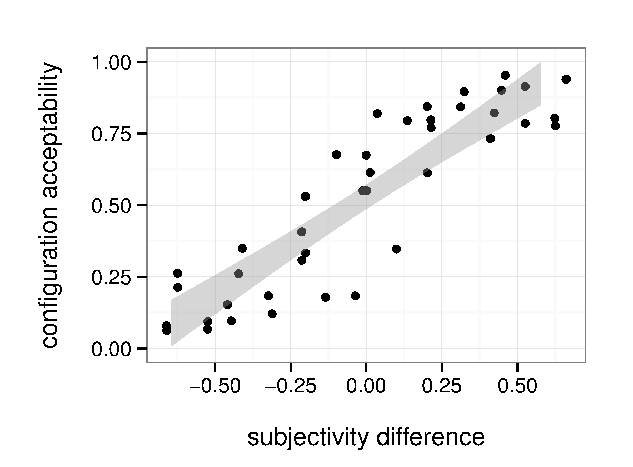
\includegraphics[width=\linewidth]{plots/comparison2.eps}
	\caption{Class-level order preferences plotted against faultless disagreement (i.e., subjectivity) difference scores.}\label{faultless-order}
\end{figure}


